% !TEX root = ../SANER2027-main-labeling.tex
% Author revisions: blue (\fixed). Coauthor revision, 2026-09-21: magenta (\coauthor).
% Issue-level resampling done (2026-09-24); configuration-selection audit still pending.

\section{Evaluation}
\label{sec:evaluations}

In this section, we present the results of our experiments and answer the four research questions posed in \Cref{sec:01_intro}, one per subsection.
\fixed{Throughout this section, a method's \emph{best} $k$ or configuration is the one with the highest macro $F_1$.}
\fixed{\Cref{fig:kcurves} reports macro $F_1$ across the $k$ grid for the three retrieval-based methods, and \Cref{tab:results} lists every method at its best configuration, including the per-class precision and recall that RQ1--RQ4 refer to.}

% Presentation pass (2026-09-22): the eight floats of the previous draft (five figures,
% three tables) are consolidated into four: the k-curve figure and the master table
% below (full width, placed at the top of the section), the per-project heatmap (RQ4,
% now column width) and the CI table (RQ4). An error-profile figure (bug/question P-R
% planes, figures/error_profile.pdf) was drafted and dropped as redundant with the table.
% The +VOTAG (fallback) macro F1 column was moved out of the master table; the CI
% table's +VOTAG rows report the fallback as differences (author decision, 2026-09-22).
% Generators: scripts/paper/fig_kcurves.py, tab_results_master.py,
% fig_per_project_diff.py, tab_method_comparison_ci.py; all read paper/tables/*.csv
% and run on any machine.
\begin{figure*}[!t]
    \centering
    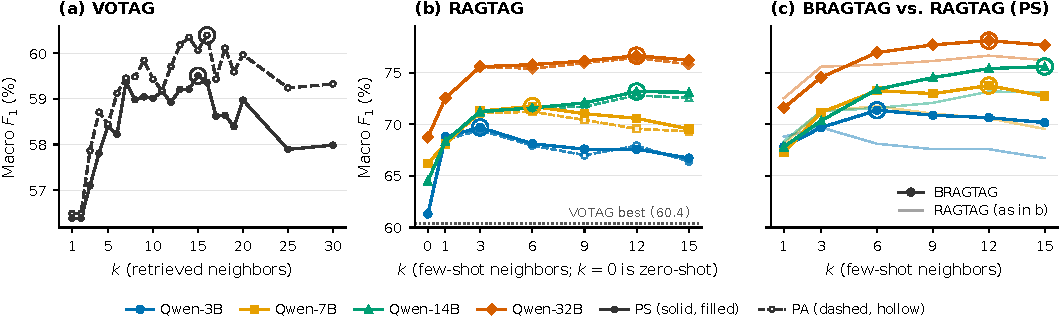
\includegraphics[width=\textwidth]{figures/kcurves.pdf}
    \caption{\fixed{Macro $F_1$ across the $k$ grid. \textbf{(a)}~\votag\ in PS (solid) and PA (dashed). \textbf{(b)}~\ragtag\ for the four Qwen sizes in PS (solid, filled) and PA (dashed, hollow). \textbf{(c)}~\bragtag\ (markers) against \ragtag. (b) and (c) share one $y$-axis and \fixed{rings} mark each method's best $k$.}}
    \label{fig:kcurves}
\end{figure*}
% Generated by scripts/paper/tab_results_master.py -- do not edit by hand.
\begin{table*}[!t]
  \centering
  \caption{Pooled test-set results of every method at its best configuration.}
  \label{tab:results}
  \footnotesize
  \renewcommand{\arraystretch}{0.97}
  \setlength{\tabcolsep}{6pt}
  \begin{tabular}{@{}llrrrrrrrrrrr@{}}
    \toprule
    Model & Method & $k$ & \multicolumn{2}{c}{Bug} & \multicolumn{2}{c}{Feature} & \multicolumn{2}{c}{Question} & $P_{\text{mac}}$ & $R_{\text{mac}}$ & Macro $F_1$ & Invalid \\
    \cmidrule(lr){4-5}\cmidrule(lr){6-7}\cmidrule(lr){8-9}
     & & & $P$ & $R$ & $P$ & $R$ & $P$ & $R$ & & & & (\%) \\
    \midrule
    -- & \votag\ (PS) & 15 & 0.552 & 0.734 & 0.677 & 0.562 & 0.592 & 0.498 & 0.607 & 0.598 & 0.595 & 0.0 \\
     & \votag\ (PA) & 16 & 0.556 & 0.731 & 0.689 & 0.579 & 0.600 & 0.508 & 0.615 & 0.606 & 0.604 & 0.0 \\
    \midrule
    Qwen-3B & Zero-shot & 0 & 0.543 & 0.915 & 0.886 & 0.610 & 0.568 & 0.353 & 0.666 & 0.626 & 0.613 & 0.2 \\
     & \ragtag\ (PS) & 3 & 0.638 & 0.803 & 0.794 & 0.813 & 0.694 & 0.494 & 0.709 & 0.703 & 0.697 & 0.2 \\
     & \bragtag\ (PS) & 6 & 0.723 & 0.665 & 0.794 & 0.813 & 0.644 & 0.646 & 0.720 & 0.708 & \textbf{0.714} & 1.8 \\
     & Fine-Tune (PS) & -- & 0.606 & 0.870 & 0.770 & 0.792 & 0.793 & 0.400 & 0.723 & 0.687 & 0.676 & 1.1 \\
     & Fine-Tune (PA) & -- & 0.637 & 0.873 & 0.833 & 0.751 & 0.724 & 0.511 & 0.731 & 0.712 & 0.708 & 0.8 \\
    \midrule
    Qwen-7B & Zero-shot & 0 & 0.575 & 0.881 & 0.792 & 0.789 & 0.783 & 0.367 & 0.717 & 0.679 & 0.662 & 0.1 \\
     & \ragtag\ (PS) & 6 & 0.657 & 0.824 & 0.787 & 0.848 & 0.838 & 0.474 & 0.761 & 0.715 & 0.718 & 3.5 \\
     & \bragtag\ (PS) & 12 & 0.713 & 0.774 & 0.761 & 0.855 & 0.825 & 0.558 & 0.766 & 0.729 & 0.738 & 3.8 \\
     & Fine-Tune (PS) & -- & 0.653 & 0.635 & 0.759 & 0.769 & 0.619 & 0.627 & 0.677 & 0.677 & 0.677 & 0.1 \\
     & Fine-Tune (PA) & -- & 0.672 & 0.878 & 0.868 & 0.825 & 0.800 & 0.588 & 0.780 & 0.764 & \textbf{0.762} & 0.3 \\
    \midrule
    Qwen-14B & Zero-shot & 0 & 0.570 & 0.876 & 0.761 & 0.855 & 0.873 & 0.294 & 0.735 & 0.675 & 0.645 & 0.1 \\
     & \ragtag\ (PS) & 12 & 0.651 & 0.844 & 0.839 & 0.836 & 0.855 & 0.489 & 0.782 & 0.723 & 0.732 & 4.5 \\
     & \bragtag\ (PS) & 15 & 0.696 & 0.803 & 0.836 & 0.844 & 0.832 & 0.579 & 0.788 & 0.742 & 0.756 & 4.7 \\
     & Fine-Tune (PS) & -- & 0.700 & 0.740 & 0.828 & 0.692 & 0.609 & 0.669 & 0.712 & 0.700 & 0.704 & 0.3 \\
     & Fine-Tune (PA) & -- & 0.730 & 0.865 & 0.882 & 0.781 & 0.764 & 0.710 & 0.792 & 0.785 & \textbf{0.785} & 0.0 \\
    \midrule
    Qwen-32B & Zero-shot & 0 & 0.611 & 0.861 & 0.766 & 0.869 & 0.857 & 0.387 & 0.745 & 0.706 & 0.688 & 0.2 \\
     & \ragtag\ (PS) & 12 & 0.701 & 0.828 & 0.855 & 0.828 & 0.840 & 0.598 & 0.799 & 0.752 & 0.767 & 4.6 \\
     & \bragtag\ (PS) & 12 & 0.748 & 0.804 & 0.847 & 0.833 & 0.808 & 0.664 & 0.801 & 0.767 & \textbf{0.781} & 4.0 \\
     & Fine-Tune (PS) & -- & 0.744 & 0.700 & 0.814 & 0.825 & 0.665 & 0.694 & 0.741 & 0.740 & 0.740 & 0.1 \\
     & Fine-Tune (PA) & -- & 0.689 & 0.929 & 0.832 & 0.876 & 0.895 & 0.534 & 0.805 & 0.780 & 0.771 & 0.1 \\
    \bottomrule
  \end{tabular}
  \par\vspace{2pt}
  \parbox{\textwidth}{\scriptsize PS: 300 labeled issues of the target project; PA: the 3{,}300 issues of all eleven projects. $P$/$R$: precision/recall; $P_{\text{mac}}$/$R_{\text{mac}}$: their macro averages. Invalid outputs count as incorrect. Bold: best macro $F_1$ per model size.}
\end{table*}


\subsection{RQ1: Effectiveness of Retrieval-Only IRC}
\label{sec:rq1}

\coauthor{We evaluate \votag\ in PS and PA at $k\in\{1,\ldots,20,25,30\}$ (\Cref{fig:kcurves}a). Similarity-weighted voting achieves its highest observed macro $F_1$ of 59.5\% at $k{=}15$ in PS and 60.4\% at $k{=}16$ in PA. Beyond these peaks, macro $F_1$ declines up to $k{=}30$. PA has slightly higher scores at every evaluated $k$. The small performance difference is consistent with the substantial overlap between retrieved neighbors: PS and PA share 84--90\% of their top-$k$ neighbors for the evaluated values between 3 and 30. Thus, even when the retrieval index includes all 3{,}300 training issues, most retrieved neighbors belong to the query's project.}

\coauthor{Question has the lowest class-specific $F_1$ at every evaluated $k$ in both settings. At the peak configurations, 32\% of question issues are predicted as bugs in both settings, compared with 18\% predicted as features in PS and 17\% in PA. Bug recall exceeds precision at every evaluated $k$, indicating that \votag\ over-predicts this class. At the peak configurations, bug recall is about 73\% and precision is 55--56\% (\Cref{tab:results}).}

\begin{coauthoranswer}
\coauthor{Retrieval-only voting achieves peak macro $F_1$ scores of 59.5\% with project-specific data and 60.4\% with pooled data. The small difference accompanies substantial overlap between retrieved neighbors. Question is the weakest class and is most often misclassified as bug.}
\end{coauthoranswer}

\subsection{RQ2: Effectiveness of Retrieval-Augmented Few-Shot IRC}
\label{sec:ragtag}

\coauthor{We evaluate \ragtag\ at $k\in\{0,1,3,6,9,12,15\}$ in PS and PA, where $k{=}0$ is the zero-shot baseline~\cite{colavito2025benchmarking}. \votag's peaks at $k{=}15$--16 (RQ1) set the upper end of this grid. \Cref{fig:kcurves}b reports macro $F_1$ across the grid in both settings.}

\coauthor{PS has slightly higher macro $F_1$ than PA at almost every (model, $k$) \fixed{pair} with $k{\ge}1$, using 300 in-project examples rather than a pool of 3{,}300. This small gap is consistent with the neighbor overlap in RQ1. Zero-shot predictions use no retrieval and are identical between settings. Below, \ragtag\ uses PS.}

\coauthor{All 48 nonzero-$k$ configurations, spanning four model sizes and both data scopes, outperform the corresponding zero-shot baseline and the strongest \votag\ configuration in macro $F_1$, macro precision, and macro recall. Thus, LLM classification using retrieved examples outperforms similarity-weighted voting. Within the PS grid, the \fixed{best $k$ is 3, 6, 12, and 12} for Qwen-3B, -7B, -14B, and -32B, respectively. These configurations achieve 69.7--76.7\% macro $F_1$, 7.6 points above zero-shot on average. Increasing $k$ from 12 to 15 does not improve any model's PS score.}

\coauthor{Question remains the weakest class by $F_1$ at every evaluated $k$ in both settings. It has the lowest recall but never the lowest precision. At zero-shot, 46--59\% of true-question issues are predicted as bugs, compared with 5--16\% predicted as features. These question-to-bug errors account for roughly 80\% of false bug predictions, linking the question-recall deficit to low bug precision.}

\coauthor{Retrieved examples reduce this confusion. At the best PS configurations, 26--36\% of question issues are predicted as bugs and 9--15\% as features. Averaged across the four models, the share of issues predicted as bug falls from 51\% to 42\%, bug precision increases from 57\% to 66\%, and question recall from 35\% to 51\% relative to zero-shot (\Cref{tab:results}). The increase in question-class $F_1$ accounts for 56--70\% of the macro-$F_1$ improvement across model sizes.}

\coauthor{The zero-shot results show that question-to-bug confusion exists before any examples are presented. We hypothesize that bug-labeled examples retrieved for true-question queries reinforce this tendency.} Based on this intuition, we propose a more balanced retrieval technique as an intervention that removes the bug-labeled neighbors whenever the query is a suspected question. We base the suspicion signal on the nearest neighbors' label distribution and calibrate it without including the test set. From each project's total 300 training issues, we assign 30 issues stratified by label as queries and 270 as the retrieval index, mirroring the PS setting. On this validation split, true-question queries retrieve almost balanced bug and question examples: averaged across $k\in[1,15]$, the mean of $N_\text{bug} - N_\text{question}$ is $-1.36$. We therefore treat a query as a suspected question when $N_\text{bug} - N_\text{question} \le m$, where $N_\text{label}$ is the count of neighbors with that label in the top-$k$ and $m$ is a small positive margin. Sweeping $m\in\{1,2,3,4,5\}$\footnote{We cap the sweep at $m{=}5$, since it is the 95th percentile of $N_\text{bug} - N_\text{question}$ on true-question queries.} on the validation split and averaging across $k\in[1,15]$, $m{=}3$ had a more favorable trade-off against the other values, firing for 89.1\% of true-question and 56.7\% of true-bug queries. We adopt $m{=}3$ and refer to the resulting method as \textbf{B}alanced \ragtag\ (\bragtag).

\begin{coauthoranswer}
\coauthor{Retrieved examples improve macro $F_1$, macro precision, and macro recall over zero-shot prompting and retrieval-only voting in every evaluated configuration with $k{\ge}1$. The best PS configurations achieve 69.7--76.7\% macro $F_1$. Question recall remains the principal weakness: 26--36\% of question issues are still classified as bugs, motivating the balanced retrieval intervention evaluated in RQ3.}
\end{coauthoranswer}

\subsection{RQ3: Effectiveness \fixed{and Trade-offs} of the Balanced Retrieval Method}
\label{sec:bragtag}

\coauthor{We compare \bragtag\ with \ragtag\ under PS at the same $k\in\{1,3,6,9,12,15\}$. At every tested $k\ge6$, \bragtag\ has higher macro $F_1$ for all four model sizes (\Cref{fig:kcurves}c)\fixed{, by at least 1.2 points}. At $k{=}1$ and $k{=}3$, its scores are lower by up to 1.0 point. With the fixed margin $m{=}3$, the condition $N_{\mathrm{bug}}-N_{\mathrm{question}}\le3$ holds for every query at these two small $k$ values. Bug-example removal is therefore unconditional, leaving no demonstrations for 40\% of queries at $k{=}1$ and 18\% at $k{=}3$.}

\coauthor{Comparing each method's best configuration, \bragtag\ increases macro $F_1$ by 1.5--2.4 points (\Cref{tab:results}).} \fixed{The 95\% CIs of these gains exclude zero for all four models, with lower bounds of 0.2--1.4 points}\footnote{1{,}000 paired bootstrap resamples per model.}. \fixed{\bragtag's} \coauthor{selected $k$ increases for the three smaller models and remains 12 for Qwen-32B.} When the trigger fires, \bragtag\ removes all bug examples from the top-$k$, so a higher initial $k$ is needed to leave enough context for the LLM.

\coauthor{The class-level results expose the trade-off. Question $F_1$ increases by 3.0--6.8 points, as recall rises by 6.5--15.3 points while precision falls by 1.2--5.0. Bug precision increases by 4.5--8.6 points, but bug recall decreases by 2.5--13.8 at every model size. The largest recall loss occurs for Qwen-3B, from 80.3\% to 66.5\%\fixed{, the one model where the intervention over-corrects}; its bug $F_1$ falls from 71.1\% to 69.3\%. Bug $F_1$ improves for the three larger models. Feature $F_1$ changes by \fixed{at most} 1.2 points. The full precision and recall values appear in \Cref{tab:results}.}

\coauthor{At these configurations, question-to-bug error rates decrease from 26--36\% with \ragtag\ to 19--27\% with \bragtag. Question-to-feature error rates change by at most 1.4 percentage points.} Averaged across $k\in[1,15]$, the question-to-bug rate drops from 31--40\% to 24--36\%. \fixed{The improvement is therefore a targeted reduction of question-to-bug confusion, at the cost of bug recall.} \coauthor{Invalid outputs remain counted as incorrect; their rates at these same configurations are reported in \Cref{tab:results} and analyzed in RQ4.}

\begin{myboxi}
\fixed{\bragtag\ outperforms \ragtag\ at every $k{\ge}6$ for all four model sizes. The gain is a targeted reduction of question-to-bug misclassifications: question $F_1$ rises by 3.0--6.8 points and bug precision by 4.5--8.6, at the cost of bug recall. Bug $F_1$ improves for the three larger models and drops by 1.8 points for Qwen-3B; feature $F_1$ changes by at most 1.2 points.}
\end{myboxi}

%\subsection{RQ4. Can retrieval-augmented few-shot prompting match LoRA fine-tuning for IRC, and what are the costs of each approach?}
\subsection{RQ4: Few-Shot Prompting vs. LoRA Fine-Tuning for IRC}
\label{sec:method-comparison}

% RQ4 rewrite (2026-09-19): five-step argument (same data -> best-vs-best ->
% error profile -> recall/invalid outputs -> fallback). TOST removed
% by author decision; paired bootstrap CIs only. All new text is blue (\fixed).
%
% Coauthor pass (2026-09-21, magenta \coauthor) reviewed 2026-09-22:
%   kept     invalid-output paragraph, fallback-protocol paragraph, fallback
%            results paragraph, CI table (now single-column), ext-table caption
%            detail on the fallback k values.
%   merged   PS/PA paragraph (0.060 rounding, PA confound, panel (b) sentence),
%            annotation-budget caveat, class-share caveat.
%   reverted section title, error-profile paragraph (author blue version),
%            "best observed" -> "best" (defined once in the S5 opener).
%   removed  encoder baselines (SetFit/RoBERTa) pending a separate decision;
%            tables/encoder_baselines.tex stays on disk but is not input.
%   cost     restored to the author's one-sentence version from c91bc26; the
%            coauthor's cost table and time discussion are dropped (not input).

%%%%%%%%%%%
\myparagraph{Classification Performance}

\fixed{We fine-tune all four models under both data scopes and compare them with \ragtag\ and \bragtag\ at their best $k$ (\Cref{tab:results}). When all methods use the same 300 labeled issues per project (PS), both retrieval-based approaches outperform fine-tuning at every model size: \ragtag\ leads by 2.1--4.0 points of macro $F_1$, and \bragtag\ by 3.8--6.0 points. Fine-tuning benefits from pooling the 3{,}300 labeled issues across all eleven projects (PA), which changes both the number of training examples and their project composition. Pooling raises its macro $F_1$ by 3.1--8.4 points relative to PS, consistent with prior findings~\cite{heo2025study}, although the class-level effects vary: for Qwen-32B, it increases bug recall but lowers question recall (\Cref{tab:results}).}

\fixed{The larger pool does not provide a corresponding benefit for retrieval (\Cref{sec:ragtag}). We therefore use PS for \ragtag\ and \bragtag\ and PA for fine-tuning in the remaining comparisons, giving each method its better-performing data scope. The eleven PS indexes collectively hold the same 3{,}300 training issues as the PA training set, so the two scopes differ in the data available per target project, not in the total annotation budget.}

% Generated by scripts/paper/tab_method_comparison_ci.py from paper/tables/method_comparison_ci.csv
% -- do not edit by hand. See the CSV header for the provenance of the current numbers.
\begin{table}[!t]
  \centering
  \caption{Macro-$F_1$ difference from PA fine-tuning in percentage points, without and with the \votag\ fallback (paired bootstrap 95\% CI).}
  \label{tab:method-comparison-ci}
  \footnotesize
  \setlength{\tabcolsep}{3pt}
  \begin{tabular}{@{}lrlrl@{}}
    \toprule
     & \multicolumn{2}{c}{\ragtag\ $-$ Fine-Tune} & \multicolumn{2}{c}{\bragtag\ $-$ Fine-Tune} \\
    \cmidrule(lr){2-3}\cmidrule(lr){4-5}
    Model & $\Delta F_1$ & 95\% CI & $\Delta F_1$ & 95\% CI \\
    \midrule
    Qwen-3B & $-1.1$ & $[-2.8, +0.7]$ & $+0.5$ & $[-1.2, +2.4]$ \\
    \quad +\votag & $-1.5$ & $[-3.2, +0.2]$ & $+0.9$ & $[-0.8, +2.8]$ \\
    \addlinespace[1.5pt]
    Qwen-7B & $\mathbf{-4.4}$ & $[-5.9, -2.9]$ & $\mathbf{-2.4}$ & $[-3.9, -0.9]$ \\
    \quad +\votag & $\mathbf{-3.3}$ & $[-4.7, -1.7]$ & $-1.1$ & $[-2.6, +0.4]$ \\
    \addlinespace[1.5pt]
    Qwen-14B & $\mathbf{-5.4}$ & $[-6.8, -3.9]$ & $\mathbf{-2.9}$ & $[-4.4, -1.3]$ \\
    \quad +\votag & $\mathbf{-4.0}$ & $[-5.4, -2.5]$ & $-1.4$ & $[-3.0, +0.1]$ \\
    \addlinespace[1.5pt]
    Qwen-32B & $-0.5$ & $[-2.0, +0.9]$ & $+1.0$ & $[-0.5, +2.4]$ \\
    \quad +\votag & $+0.8$ & $[-0.8, +2.2]$ & $\mathbf{+2.1}$ & $[+0.6, +3.5]$ \\
    \midrule
    All sizes & $\mathbf{-2.8}$ & $[-3.9, -1.8]$ & $-1.0$ & $[-2.0, +0.1]$ \\
    \quad +\votag & $\mathbf{-2.0}$ & $[-3.0, -1.0]$ & $+0.1$ & $[-0.9, +1.1]$ \\
    \bottomrule
  \end{tabular}
  \par\vspace{2pt}
  \parbox{\columnwidth}{\scriptsize \ragtag/\bragtag\ under PS at their best $k$, fine-tuning under PA; negative values favor fine-tuning. Each +\votag\ row applies the \votag\ fallback for invalid outputs to both methods. Bold: CI excludes zero. All sizes: mean of the four per-model differences.}
\end{table}


\fixed{\Cref{tab:method-comparison-ci} reports macro $F_1$ differences as the retrieval-based method minus fine-tuning, with paired bootstrap 95\% CIs.\footnote{We use 1{,}000 paired bootstrap resamples per comparison.} Averaged over the four model sizes, \ragtag\ trails fine-tuning by 2.8 points, and \bragtag\ trails it by 1.0 point, a gap whose CI includes zero. \ragtag\ trails fine-tuning at every model size, whereas \bragtag\ improves on \ragtag's difference at every size, to between 2.9 points behind and 1.0 point ahead. Fine-tuning is significantly ahead at Qwen-7B and Qwen-14B. At Qwen-3B and Qwen-32B, the confidence intervals include zero, and \bragtag\ has the higher point estimates. Results also vary by project: \bragtag\ matches or exceeds PA fine-tuning in 16 of the 44 (project, model) pairs, including all four sizes on \texttt{opencv} and three of four on \texttt{bitcoin} (\Cref{fig:per-project-diff}).}

\begin{figure}[!t]
    \centering
    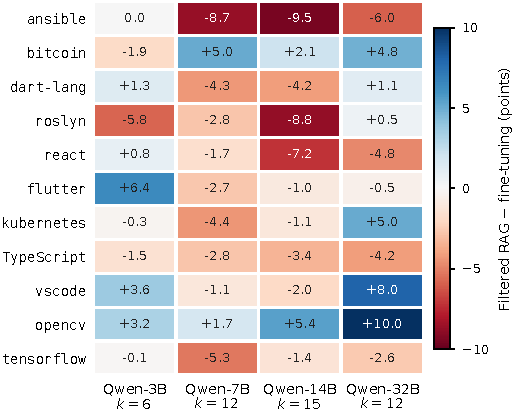
\includegraphics[width=\columnwidth]{figures/per_project_diff.pdf}
    \caption{\fixed{Macro $F_1$ difference in percentage points between \bragtag\ (PS, best $k$) and PA LoRA fine-tuning on each project's 300 test issues, for the four model sizes. Blue favors \bragtag, red favors fine-tuning.}}
    \label{fig:per-project-diff}
\end{figure}

\fixed{Fine-tuning detects more actual bugs at every model size, while \bragtag\ makes fewer false bug predictions at three of the four sizes. Like the zero-shot models (\Cref{sec:ragtag}), the PA fine-tuned models over-predict bug: they assign this label to 39--46\% of test issues, although only 33\% are bugs. Their bug recall is high (86--93\%), but precision is lower (64--73\%), and 23--36\% of question issues are classified as bugs. \bragtag\ predicts bug for 31--38\% of issues, closer to the true share, and misclassifies 19--27\% of questions as bugs. Its bug recall is lower (66--80\%), while its precision is generally higher (70--75\%). The one size at which \bragtag\ does not make fewer false bug predictions is Qwen-14B, where fine-tuning's tendency to over-predict bug is less pronounced: it labels 39.5\% of issues as bugs and misclassifies 23\% of questions as bugs. A bug share close to the true proportion is not by itself evidence of quality; what matters is the trade-off between bug recall and bug precision, and which method is preferable depends on the relative cost of missed bugs and incorrect bug assignments in a given project.}

\coauthor{At Qwen-7B and Qwen-14B, \bragtag's macro recall is lower than LoRA's by 3.5 and 4.3 points, respectively, while its macro precision is within 1.5 points of LoRA's at every size. Invalid outputs contribute to this recall deficit: they count as false negatives for the true class without adding a prediction to any valid class's precision denominator. At the selected configurations, invalid rates are 0.2--4.6\% for \ragtag, 1.8--4.7\% for \bragtag, and at most 0.8\% for LoRA. For \bragtag\ at Qwen-7B and larger sizes, 6--8\% of true bugs receive invalid outputs.}

\coauthor{We therefore compare complete pipelines that assign a valid label to every issue by applying a \votag\ fallback only when the LLM output is invalid. The fallback uses PS voting at fixed $k{=}15$ for \ragtag/\bragtag\ and PA voting at fixed $k{=}16$ for LoRA. It uses the original, unfiltered neighbors, independently of the number of demonstrations shown to the LLM. The retrieval-based pipelines can reuse their cached neighbor pool; adding this fallback to LoRA introduces a retrieval step. No additional LLM calls are required.}

\coauthor{After applying the fallback to all three LLM approaches (\Cref{tab:method-comparison-ci}, +\votag\ rows), \bragtag\ ranges from 1.4 points behind LoRA to 2.1 points ahead. Its deficits at Qwen-7B and Qwen-14B are approximately halved, to 1.1 and 1.4 points, while its Qwen-32B lead grows to 2.1 points. LoRA's scores change by at most 0.3 points.} \fixed{On average, \bragtag\ is then 0.1 points ahead of fine-tuning, with a CI that includes zero, and per model the interval excludes zero only at Qwen-32B, in \bragtag's favor.}

%%%%%%%%%%%%%%%%%%%%%
\myparagraph{Computation and Data Cost}

% \begin{figure}[t]
%     \centering
%     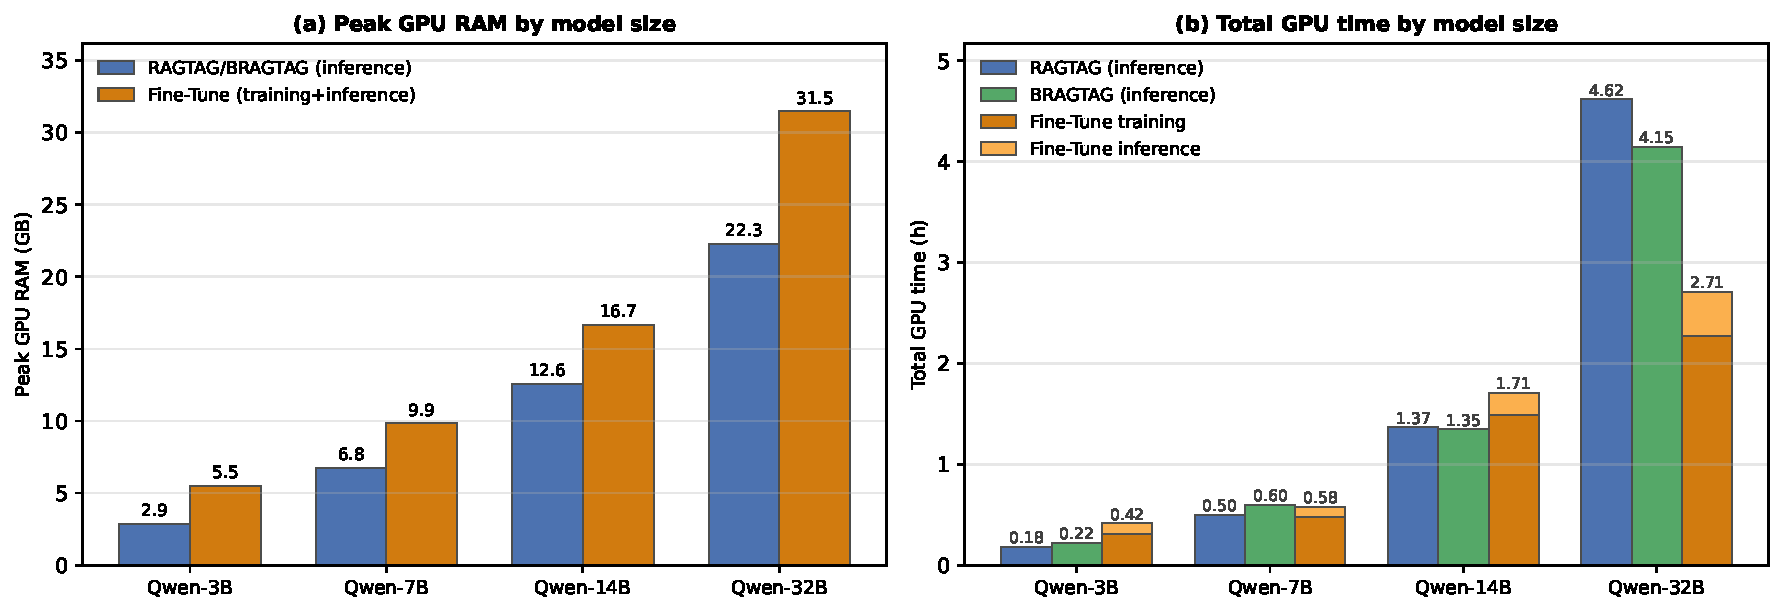
\includegraphics[width=\linewidth]{figures/cost_analysis.pdf}
% \caption{\textbf{(a)} Peak GPU memory by model size for \ragtag/\bragtag\ inference compared with LoRA fine-tuning training plus inference. \textbf{(b)} Total GPU time by model size for \ragtag\ and \bragtag\ compared with LoRA fine-tuning.}
%     \label{fig:cost-analysis}
% \end{figure}

% Author's shortened version (commit c91bc26), restored 2026-09-22; "per project"
% added to match the annotation-budget caveat earlier in this subsection.
% tables/method_cost.tex input again 2026-09-24, with the time trade-off below.
% Savings from peak GPU memory in GB, RAG vs. LoRA incl. training: 2.9/5.5, 6.8/9.9, 12.6/16.7, 22.3/31.5.
% VOTAG cost measured 2026-09-24 (tables/method_cost.tex header).
\begin{table}[t]
  \centering\color{blue}
  \caption{Computational cost of \ragtag, \bragtag, and LoRA fine-tuning at the configurations of \Cref{tab:method-comparison-ext}. RAM is the observed peak GPU memory; Train and Infer are wall-clock runtimes on a single GPU (\ragtag/\bragtag\ have no training phase), and Total is their sum, excluding model load.}
  \label{tab:method-cost}
  \footnotesize
  \setlength{\tabcolsep}{3.5pt}
  \begin{tabular}{llcccc}
    \toprule
    Model & Method & RAM (GB) & Train (h) & Infer (h) & Total (h) \\
    \midrule
    Qwen-3B & \ragtag & 2.9 & -- & 0.18 & 0.18 \\
     & \bragtag & 2.9 & -- & 0.22 & 0.22 \\
     & Fine-Tune & 5.5 & 0.31 & 0.11 & 0.42 \\
    \addlinespace[2pt]
    Qwen-7B & \ragtag & 6.8 & -- & 0.50 & 0.50 \\
     & \bragtag & 6.8 & -- & 0.60 & 0.60 \\
     & Fine-Tune & 9.9 & 0.48 & 0.10 & 0.58 \\
    \addlinespace[2pt]
    Qwen-14B & \ragtag & 12.6 & -- & 1.37 & 1.37 \\
     & \bragtag & 12.6 & -- & 1.35 & 1.35 \\
     & Fine-Tune & 16.7 & 1.49 & 0.22 & 1.71 \\
    \addlinespace[2pt]
    Qwen-32B & \ragtag & 22.3 & -- & 4.62 & 4.62 \\
     & \bragtag & 22.3 & -- & 4.15 & 4.15 \\
     & Fine-Tune & 31.5 & 2.28 & 0.44 & 2.71 \\
    \bottomrule
  \end{tabular}
\end{table}


\fixed{Our RAG-based methods require 47\%, 31\%, 25\%, and 29\% less peak GPU memory than LoRA fine-tuning for Qwen-3B, -7B, -14B, and -32B, respectively (33\% on average), while using $11\times$ less labeled data per project (\Cref{tab:method-cost}). They have no training phase, but their inference takes longer. Fine-tuned models label the 3{,}300 test issues in 0.10--0.44~h, whereas \ragtag\ and \bragtag\ take 0.18--4.62~h. Including training, \bragtag\ takes less total time than fine-tuning at Qwen-3B and Qwen-14B, about the same at Qwen-7B, and more at Qwen-32B (4.15~h versus 2.71~h). Without an LLM, \votag\ labels the 3{,}300 test issues in under 4~s with 0.2~GB of GPU memory, at a macro $F_1$ of 59.5\% (\Cref{sec:rq1}).}

\begin{myboxi}
% \textbf{Answer to RQ4:} 
\fixed{Averaged over the four model sizes, \bragtag\ with only the target project's labeled issues achieves a macro $F_1$ statistically indistinguishable from that of fine-tuning on all eleven projects' labeled issues, while needing no training, $11\times$ less labeled data per project, and 33\% less peak GPU memory. Per model size, the difference is significant only at Qwen-7B and Qwen-14B, in fine-tuning's favor, and, with a \votag\ fallback for invalid outputs, only at Qwen-32B, in \bragtag's favor. Without balancing, \ragtag\ trails fine-tuning by 2.8 points on average. When fine-tuning also uses only the target project's labeled issues, \ragtag\ and \bragtag\ score higher than it at every model size. Fine-tuning detects more bugs but over-predicts the bug class, whereas \bragtag\ makes fewer false bug predictions.}
\end{myboxi}
